These are lecture notes from the Active Matter course held at Göttine University in the summer semester.
The lectures are by Benoît Mahault and Ramin Golestanian of the Max Planck Insitute of Dynamics and Self-Organization, featuring a range of guest lecturers, and the notes are typeset by Martin Kjøllesdal Johnsrud.
The notes meant to give a short introduction to the Active Matter course, and present some background material in the form of concepts and mathematical tools that are often used to apprehend active systems.

% Handwritten page I 


\subsection{What is active matter?}

\todo[inline]{Re-draw figures}

As widely accepted definition of active matter consists to say that it is made of elementary units that locally dissipate energy in a continuous and sustained manner. Hence, the dynamics of active particles break time-reversal symmetry, \textit{it is inherently far from thermodynamic equilibrium}. In many cases, activity manifests as persistent motion, but can also take the form of local production of forces, sustaining of chemical reactions, growth (reproduction), or several of them at the same time. This definition is very broad and encompasses a multitude of biological examples spanning many scales:

\begin{figure}[!htb]
    \centering
    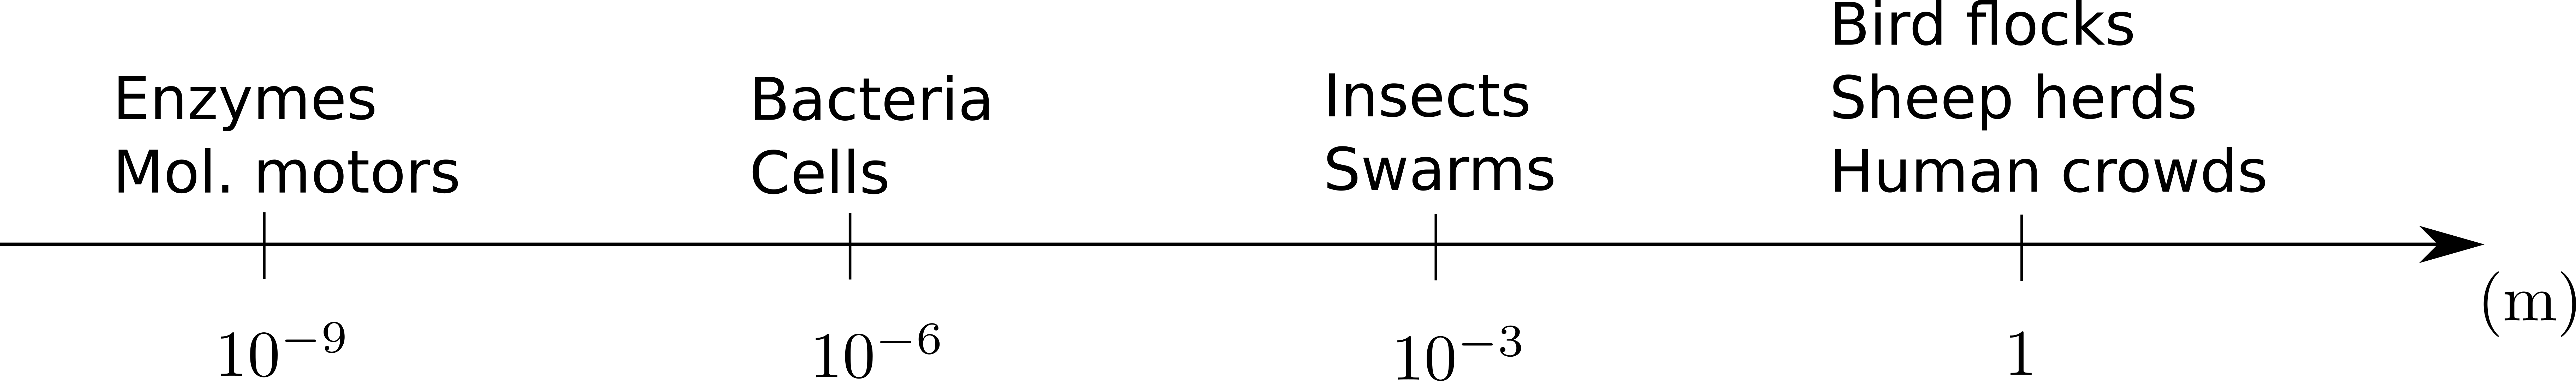
\includegraphics[width=.8\textwidth]{Figures/introduction/scales.png}
    \caption{The range of scales of active particles.}
    \label{fig: scales active particles}
\end{figure}


% Handwritten page II

\begin{itemize}
    \item Enzymes, molecular motors (nm): Enzymes (E) catalyze chemical reactions of a substrate (S),
    %
    \begin{align}
        E + S \longrightarrow  \underbrace{SE}_{\mathrm{binding}} \longrightarrow  E + P
    \end{align}
    %
     and thus locally generate chemical gradients, $\bm \nabla P$. 
     \begin{figure}[H]
        \centering
        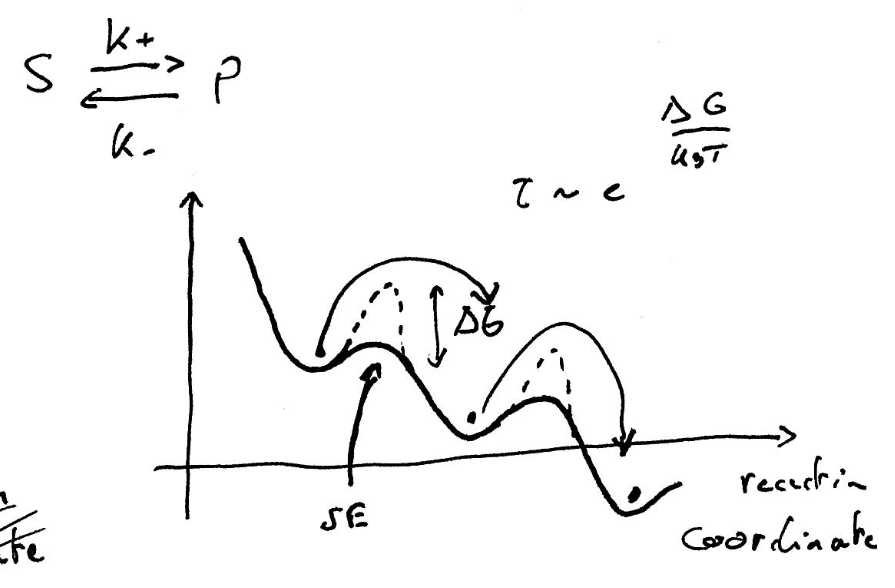
\includegraphics[width=.3\textwidth]{Figures/introduction/enzymes.png}
        \caption{The energy landscape for the chemical reaction is modified by the }
        \label{fig: enzymes}
    \end{figure}
     Molecular motors couple chemical cycles to displacements or rotations, so that these molecular machines can exhibit self-propulsion.\\
     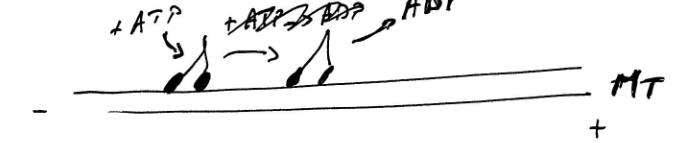
\includegraphics[width=.3\textwidth]{Figures/introduction/motors.png}
    \item Bacteria, cells ($\mu$m): Bacteria and algae usually move thanks to filamentous appendices called flagella or cilia, which are powered by molecular motors.
    \\
    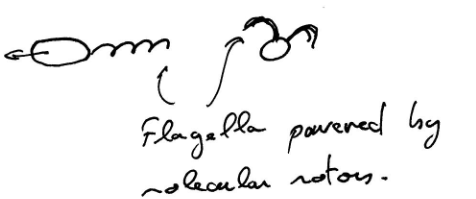
\includegraphics[width=.3\textwidth]{Figures/introduction/bacteria.png} 
    \\
    Another example is cells that self-propel on the substrate by polymerizing actin filaments at their front.
    \\
    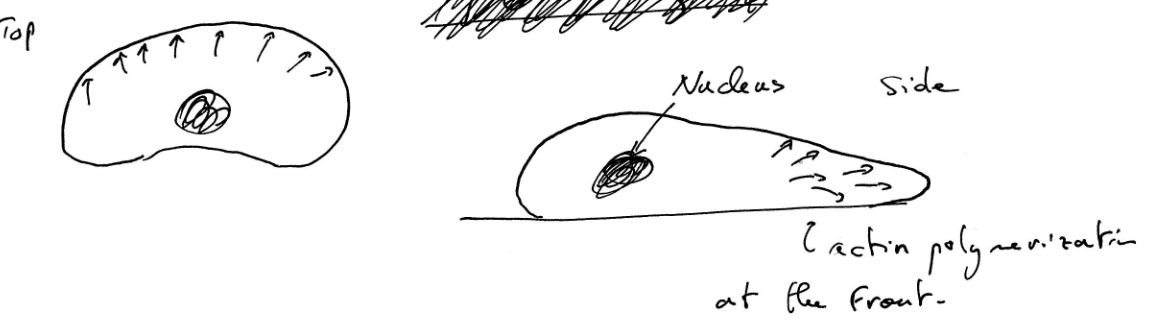
\includegraphics[width=.25\textwidth]{Figures/introduction/actin.png}
    \item Insect swarms (mm)
    \item Animal herds, human crowds (m)
\end{itemize}


% Handwritten page III

\subsection{What makes active matter special?}

Active systems, because they constantly dissipate energy in their bulk, and in contrast to passive systems globally driven (turbulence, shaken granulars, \ldots), are able to spontaneously self-organize and create macroscopic structures. 
Again, these ideas are relevant to many examples in the living world including the architecture of the cytoskeleton, the morphogenesis of multicellular organisms, or the collective motion arising from social interactions in groups of several hundred or thousands of individuals. 

Active matter is also not restricted to the study of biological systems, as the design and study of synthetic active particles now represent a large part of the field. Those allow for better controlled experiments and often exhibit similar phenomenology as their biological counterpart, thus opening the way to biomimetic materials engineering. 
\todo[noinline]{Notorious? isn't that a bit negative?}
Notorious examples of artificial active matter include assemblies of self-propelled colloids (Phoretic Janus particles, Quincke rollers), artificial microswimmers (self-propelled drops, magnetic swimmers), and robots.

\begin{figure}[!htb]
    \centering
    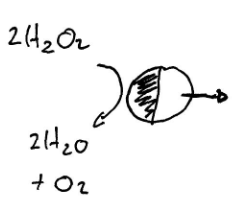
\includegraphics[width=.3\textwidth]{Figures/introduction/janus.png}
    \caption{A self-propelled Janus particle, to be discussed in Lecture 7}
    \label{fig: janus}
\end{figure}
\todo[noinline]{Give ref}



\subsection{On the nonequilibriumness of active assemblies}

As written above, active matter is inherently `far' from equilibrium, since it is assembled from particles whose dynamics constantly break time-reversal symmetry. This means that active systems lack many of the properties familiar to equilibrium systems. These include:
%
\begin{enumerate}
    \item Absence of minimization principle: active dynamics are not constrained by the second law, so that they do not converge over long times to a state with maximal entropy (or minimum free energy). In fact, whether an active system converges to a steady state or not is a priori unknown.
    \item No time-reversal symmetry: as a consequence of 1, active systems can (and do) generally produce macroscopic currents, leading to phases where TRS is collectively broken.
    \item Lack of thermodynamic framework: Basic equilibrium concepts such as temperature or thermodynamic pressure are usually not defined for active systems. Additionally, active systems generally do not exhibit an equation of state, meaning that their bulk properties are not only determined by their material properties but can also be substantially affected by the nature and shape of the container they live in.
    \item Memory: again, due to 1 and contrary to systems at equilibrium, the state of an active system may be dependent of its past history.
    \item In active matter, momentum is not conserved so that forces do not necessarily need to satisfy the action-reaction principle. Familiar examples of such `nonreciprocity' are encountered in predator-prey systems, while it also generally arises when particles interact via self-generated fields such as bacteria or phoretic colloids.
\end{enumerate}
%
In summary, the collective behaviours found in active systems thus generally break our intuition built on equilibrium physics, and their theoretical understanding requires to use and develop specifically tailored tools and concepts.
In particular, we will construct field theory descriptions of active systems, such as IRR thermodynamics\todo{Irrecersible thermodynamics?} and performe coarse-graining using kinetic theory.\todo[noinline]{Is this right?}


% Handwritten Page IV

\subsection{The idea of this course}

Active matter is very large and quickly developing field borrowing tools and concepts from various other areas of physics including soft matter, biological physics, hydrodynamics, and statistical physics. So, this course is only meant as an introduction to the basics of the very diverse phenomenology of active systems, and how it is usually apprehended. In particular, our journey will be driven by two general aspects which are still the topic of active research:
\begin{itemize}
    \item How is active motion generated at the micro scale, and what are its consequences on the dynamics of active particles?
    \item How do active systems convert energy dissipated at the molecular scale into the formation of structure and order macroscopic scales?
\end{itemize}
These two lectures is meant to give an overview of the topic that will be addressed in the following weeks, while we will also introduce useful concepts and mathematical tools.



% Handwritten page V

\section{Hydrodynamics of microswimmers}

Many active particles evolve in a fluid, which they need to displace in order to move. Understanding the locomotion of such swimmers thus requires to study the dynamics of the flow around them. The fluid surrounding the particles is generally incompressible so that it is defined by its local velocity $\bm v$ which obeys the Navier-Stokes equations:
%
\begin{subequations}
\label{eq_NS}
\begin{align}
    \label{eq_NS_v}
    \rho \left[ \partial_t \bm v + (\bm v \cdot \nabla)\bm v \right] & = \eta \nabla^2\bm v - \nabla P + \bm f, \\
    \label{eq_NS_inc}
    \nabla \cdot \bm v & = 0.
\end{align}
\end{subequations}
%
The terms on the left-hand side of~\eqref{eq_NS_v} correspond to the material derivative and simply model the effect of inertia, while on the right-hand side the first term originates from viscous dissipation, the second is the pressure which ensures incompressibility as required by~\eqref{eq_NS_inc}, while the active force $\bm f$ arises as a source term.
In cases dominated by inertia or dissipation, the NS Eq.~\eqref{eq_NS} simplifies. To understand this, let us define the typical length and velocity scales of the problem, $L$ and $V$, and apply the following rescaling:
%
\begin{equation*}
    \bm v \to V \bm v', \quad
    \bm x \to L \bm x', \quad
    t \to \frac{L}{V}t', \quad
    P \to \frac{\eta V}{L} P', \quad
    \bm f \to \frac{\eta V}{L^2} \bm f'.
\end{equation*}
%
We obtain the following equation in terms of the dimensionless primed variables
%
\begin{equation}
    {\rm Re}\left[ \partial_{t'} \bm v' + (\bm v' \cdot \nabla')\bm v' \right] = \nabla'^2\bm v' - \nabla' P' + \bm f',
\end{equation}
%
where ${\rm Re} = \rho V L / \eta$ is known as the Reynolds number. 
Alternatively, note that the Reynolds number can be obtained by the ratio of the typical scales associated with the convection ($\bm v\cdot \nabla \bm v$) and dissipation ($\eta\nabla^2\bm v$) in the Navier-Stokes equation. 
Hence, the value of the Reynolds number controls the relative importance of inertial effects and viscous dissipation.
For a micron-sized swimmer in water such as bacteria, we can evaluate $\rho \approx 10^3 \; {\rm kg / m^3}$, $\eta \approx 10^{-3} \; {\rm Pa \cdot s}$,
$V \approx 10^{-5}\; {\rm m/s}$, and $L \approx 10^{-6} \; {\rm m}$, such that ${\rm Re} \approx 10^{-5}$.
%
% Handwritten page VI
%
\textit{Microswimmers therefore evolve at vanishing Reynolds number} where inertial effects are negligible. 
Their dynamics then evolve in the so-called Stokes regime, 
such that the flow they generate obeys the Stokes equation:
%
\begin{subequations}
\label{eq_Stokes}
\begin{align}
    \label{eq_Stokes_v}
    \eta \nabla^2\bm v -\nabla P + \bm f & = \bm 0, \\
    \label{eq_Stokes_inc}
    \nabla \cdot \bm v & = 0.
\end{align}
\end{subequations}
%
Contrary to the Navier-Stokes equation, Eqs.~\eqref{eq_Stokes} do not have time derivatives and are linear.
The flow velocity $\bm v$ only therefore only depends on the instantaneous value of the force $\bm f$ (there is no inertia), and it varies linearly with it\footnote{By taking the divergence of~\eqref{eq_Stokes_v}, you can convince yourself that the pressure is also a linear function of the force.}. 
An important consequence of these features is that is that Stokes flow obey kinematic reversibility, meaning that they obey the symmetry
%
\begin{equation*}
    \bm f \rightarrow -\bm f, \qquad \bm v \rightarrow -\bm v.
\end{equation*}
%
As such, sequences of motion are reversible.
One important consequence of this is the \emph{scallop theorem}, which states that a microswimmer cannot achieve self-propulsion with reciprocal motion.
%
\begin{figure}[!htb]
    \centering
    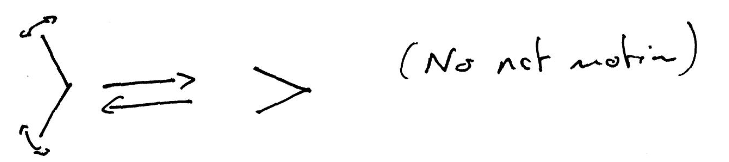
\includegraphics[width=.3\textwidth]{Figures/introduction/scallop.png}
    \caption{A scallop moves by opening and closing its shells, which in the Stokes regime gives zero net motion}
    \label{fig: scallop}
\end{figure}

The name comes from an example of reciprocal motion, a scallop opening and closing its shell
Self-propulsion therefore requires at least 2 independent degrees of freedom (d.o.f.)\todo[noinline]{I think this is not a good statement, unless dof is well defined}
Examples of this are swimmers with a corkscrew flagella or breast-stroke-like motion.
Such swimmers are force and torque-free, as the net forces/torques from the flagella and the drag adds up to zero.



\begin{figure}[!htb]
    \centering
    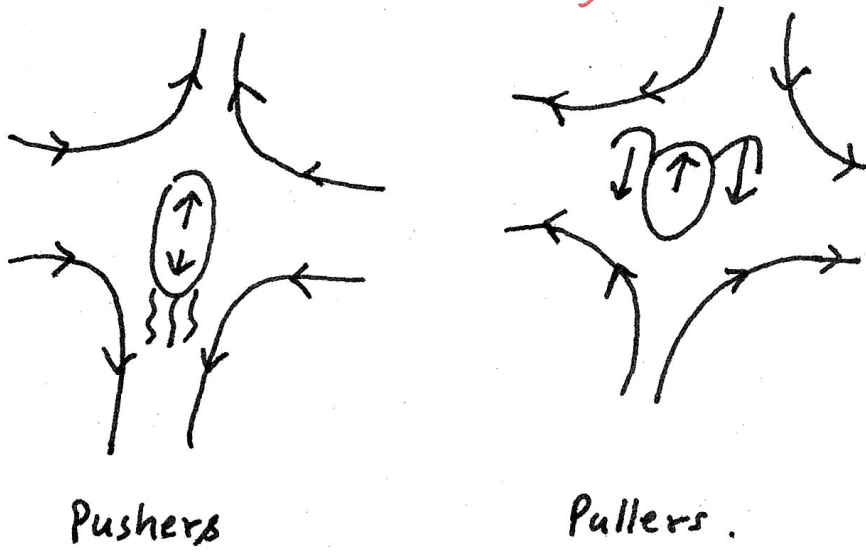
\includegraphics[width=.5\textwidth]{Figures/introduction/swimmers.png}
    \caption{Two examples of microswimmers}
    \label{fig: swimmers}
\end{figure}





% handwritten page VII

\section{A minimal model for active motion}


In the previous section, discussed by which mechanism active motion can arise (in the nontrivial context of microswimmers).
Here, we will be rather ask the question of what the consequences of the presence of a self-propulsion speed on the dynamics of an active particle are.
For this, assume that a particle is able to self-propel but we won't particularly focus on the details of its self-propulsion mechanism.


\subsection{Some basics on Brownian motion}

\begin{figure}[!htb]
    \centering
    \includegraphics[width=.25\textwidth]{Figures/introduction/brownian.png}
    \caption{A Brownian particle is constantly and randomly interacting with smaller particles.}
    \label{fig: brownian}
\end{figure}

Before discussing active motion, let us give a brief recap on the theory of Brownian motion.
Consider a micron-sized particle in a fluid at temperature $T$. 
The particle constantly undergoes collisions with the fluid molecules, and its mass is low enough that the results of such collisions result in visible erratic dynamics known as Brownian motion.
The dynamics of the particle is described by the \emph{Langevin equation}
%
\begin{equation} \label{eq_LangevinBM}
    m\frac{\rmd^2 \bm r}{\rmd t^2} + \zeta \frac{\rmd \bm r}{\rmd t} = \bm f(t).
\end{equation}
%
Equation~\eqref{eq_LangevinBM} is nothing but Newton's second law, so that the first term on the left hand side represents the acceleration of the particle multiplied by its mass, and the second term accounts for the Stokes friction exerted by the fluid in response to the motion of the particle.
In fact, the ratio of the particle mass and friction coefficient defines a timescale $\tau = m / \zeta$ beyond which inertial effects can be neglected.
For a micron-size sphere with a density comparable to that of water, we have
%
\begin{equation*}
    \tau = \frac{\rho \tfrac{4\pi}{3} R^3}{6 \pi \eta R} 
    = \frac{2\rho R^2}{9\eta} \approx 0.2 \; \mu{\rm s}.
\end{equation*}
%
Hence, for observation times beyond the micro-second inertial effects can generally be safely neglected so that we can neglect the interaction term in~\eqref{eq_LangevinBM}, which can be expressed in this overdamped limit as
\begin{equation} \label{eq_LangevinBM_ovd}
    \frac{\rmd \bm r}{\rmd t} = \frac{1}{\zeta}\bm f(t).
\end{equation}
%
The force $\bm f$ arises from the multiple collisions that the particle undergoes with the solvent molecules. 
Under the approximation that these collisions are isotropic, identically distributed and uncorrelated random events, we can use the central limit theorem to approximate the distribution of the stochastic process $\bm f$ by a normal distribution with zero mean and variance $\sigma$.
Namely, denoting averages with independent realizations of the noise with the notation $\langle \cdot \rangle$, the first two moments of the components of $\bm f$ read
\begin{equation*}
    \langle f_i(t) \rangle = 0, \qquad
    \langle f_i(t) f_j(t') \rangle = \sigma^2 \delta_{ij}\delta(t - t').
\end{equation*}

Equation~\eqref{eq_LangevinBM_ovd} can be easily solved as
\begin{equation*}
    \Delta \bm r(t) = \bm r(t) - \bm r(t=0) = \frac{1}{\zeta} \int_0^t\rmd\tau \bm f(\tau).
\end{equation*}
Solution implies that $\langle \Delta \bm r(t) \rangle = \bm 0$ and $\langle |\Delta \bm r(t)|^2 \rangle = 2 d \sigma^2 / \zeta^2 t$.
Two main features of Brownian motion (diffusion): no net motion and mean-squared displacement (MSD) grows linearly in time (diffusion coefficient is $D = \sigma^2 / \zeta^2$).
Additionally, the fluctuation-dissipation relation relates $D$ to the solvent temperature as $D = k_{\rm B}T / \zeta$. The signification of this relation is that the damping friction and fluctuations come from the same medium.

% Hand written page VIII

This problem is sufficiently simple so that one can obtain the full distribution of the particle position. 
For this, we define $\calP(\bm x,t) = \langle \delta(\bm x - \bm r(t)\rangle$, which obeys the Fokker-Planck equation:
%
\begin{equation} \label{eq_FP_BM}
    \partial_t \calP(\bm x,t) - D \nabla^2 \calP(\bm x,t) = 0
\end{equation}
%
Assuming that the particle sits at $\bm x = \bm 0$ at time $t=0$, the solution of Equation~\eqref{eq_FP_BM} is given by
\begin{equation*}
    \calP(\bm x,t) = \frac{1}{(4\pi D t)^{d/2}}e^{-\tfrac{|\bm x|^2}{4 D t}}.
\end{equation*}
We notice that the mean of the distribution is at $\bm x = \bm 0$ at all times and that the width, i.e. the standard distributions, grows as $\sqrt{t}$.


\textit{
    {\bf Homework:} Consider a Brownian particle in a potential $U$, write the associated Fokker-Planck equation. Show that the stationary solution corresponds to the Boltzmann distribution.
For a harmonic potential $U = \tfrac{1}{2} k |\bm x|^2$, the solution of the FPE is given by 
\begin{equation*}
    \calP(\bm x,t) = \left(\frac{\lambda}{2\pi D (1 - e^{-2\lambda t})}\right)^{d/2}e^{-\tfrac{\lambda}{2 D} \tfrac{|\bm x|^2}{1 - e^{-2\lambda t}}},
\end{equation*}
with $\lambda = k / \zeta$.
Calculate mean displacement and MSD, comment.
}



\subsection{Active Brownian motion}

Although we described the dynamics of a passive particle in the previous section, the Langevin description approach does not a priori assume that the particle is in equilibrium. 
Hence, we can straightforwardly generalize it by assuming that the particle is able to self-generate a force leading to an active velocity $\va$. 
Therefore, Equation~\eqref{eq_LangevinBM_ovd} now becomes
\begin{equation}\label{eq_LangevinABM}
    \frac{\rmd \bm r}{\rmd t} = \va + \frac{1}{\zeta}\bm f(t).
\end{equation}
To fully characterize the dynamics, we now need to specify how $\va$ evolves in time. 
Self-propelled motion can in fact arise in various ways, but what we argue below is that its most important feature is that $\va$ introduces a finite persistence length in the particle motion.

For example, the dynamics of bacteria like \textit{E. coli} consists of alternating sequences of `run' and `tumble', respectively corresponding to persistent motion along a fixed direction and random reorientations. 
Other active swimmers like self-propelled colloids, on the other hand, follow smooth trajectories as their direction of motion slowly diffuses in time due to thermal fluctuations.
In both cases, defining the typical particle velocity as $v_0$ and reorientation time $\tau_r$, the persistence length can be built from dimensional analysis as $\lp = v_0 \tau_r$.
Physically, this means that on length scales below $\lp$ the active particle exhibits ballistic motion with a speed $\approx v_0$, while on scales $\gg \lp$ its direction of motion has randomized and its overall dynamics is diffusive. 


\begin{figure}[!htb]
    \centering
    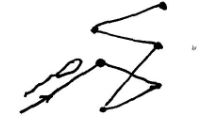
\includegraphics[width=.2\textwidth]{Figures/introduction/runandtumble.png}
    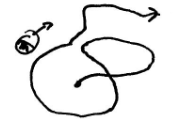
\includegraphics[width=.2\textwidth]{Figures/introduction/smooth.png}
    \caption{Run and tumble versus smooth trajectories of self-propulsion}
    \label{fig: run and tumble vs smooth}
\end{figure}

As a minimal model of active velocity, we can thus simply assume that the particle self-propels at constant speed $v_0$, while the unit vector $\he$ parametrizing its orientation is a colored noise with zero mean and exponential correlations:
\begin{equation} \label{eq_cf_e}
    \langle \he(t) \cdot \he(t + \tau) \rangle = e^{-\tau / \tau_r}.
\end{equation}


We then immediately deduce that, assuming the noise of the orientation and force is independent,
\begin{align}
    \langle |\Delta \bm r(t)|^2 \rangle & = 2 d D t 
    + v_0^2 \int_0^t\rmd\tau_1\int_0^t\rmd\tau_2 \, e^{-|\tau_1-\tau_2|/\tau_r} \nonumber \\
    & = 2 d D t 
    + 2 \lp^2 \left( \frac{t}{\tau_r} - 1 + e^{-t/\tau_r} \right).
\end{align}
%
This has two limiting regimes, much smaller and much larger times than the reorientation time,
%
\begin{align*}
    \langle |\Delta \bm r(t)|^2 \rangle & 
    \underset{t \ll \tau_r}{\simeq} 2 d D t + v_0^2 t^2 , \\
    \langle |\Delta \bm r(t)|^2 \rangle & 
    \underset{t \gg \tau_r}{\simeq} 2 d D_{\rm eff} t , \qquad  D_{\rm eff} = D + \frac{v_0^2\tau_r}{d}. 
\end{align*}
%
This corresponds to three dynamical regimes, with thermal diffusion at short times ($t < 2 d D / v_0^2)$, ballistic dynamics at intermediate times ($2 d D / v_0^2 < t < \tau_r)$ and diffusive motion at long times $t > \tau_r$. 
This confirms the qualitative picture drawn earlier, and is illustrated in \autoref{fig: MSD}.

\begin{figure}[!htb]
    \centering
    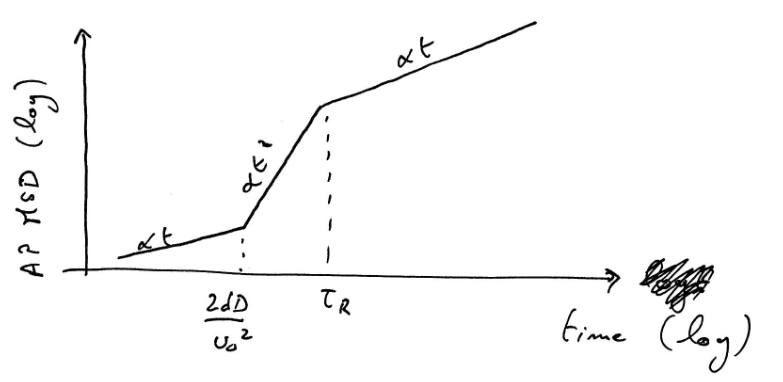
\includegraphics[width=.6\textwidth]{Figures/introduction/crossover.png}
    \caption{The mean-square displacement for different regimes}
    \label{fig: MSD}
\end{figure}




% Handwritten page 10

\subsection{Description of the long-time regime via the moment expansion}

We may recover the same result from the Fokker-Planck description.
We will consider the 2D case, in which we may write the vector parametrizing the orientation of the particle in terms of a single angle,
%
\begin{align}
    \hat {\bm e}(\theta) 
    =
    \begin{pmatrix}
        \cos \theta \\ \sin \theta
    \end{pmatrix},
\end{align}
%
where the evolution of the angle is given by a Langevin equation,
%
\begin{align}
    \odv{ \theta }{ t } = \sqrt{2 D_R} \eta_R(t).
\end{align}
%
Here, $\eta_R$ is unit white noise.
We define the probability density for the particle as before,
%
\begin{align}
    \calP(\bm r, \phi, t)
    =
    \E{\delta(\bm x - \bm r(t))\delta(\phi - \theta(t))}.
\end{align}
%
This obeys the Fokker-Planck equation
%
\begin{align}
    \partial_t \calP(\bm r, \phi, t)
    + \bm \nabla \cdot [
        v_0 \hat {\bm e}(\theta ) \calP(\bm r, \phi, t)
        - D \bm \nabla \calP(\bm r, \phi, t)
    ]
        - D_r \partial_\theta^2 \calP(\bm r, \phi, t)
        = 0.
\end{align}
%
This equation has no simple analytical solution.
However, in the regime where $t\gg 1 / D_R \equiv \tau_R$ it may be described well using \emph{moment expansion}.
This is a powerful technique is is also very useful for more complex situations.

We begin by defining the particle density,
%
\begin{align}
    \rho(\bm r, t) = \int_0^{2\pi} \dd \phi\, \calP(\bm r, \phi, t).
\end{align}
%
We may find its equation of motion by taking a time derivative, and applying the Fokker-Planck, which gives us
%
\begin{align}\label{eq: density FP}
    \partial_t \rho + v_0 \bm \nabla \cdot (\rho \bm q) - D \nabla^2 \rho = 0,
\end{align}
%
where we have defined
%
\begin{align}
    \bm q(\bm r, t)
    =
    \frac{1}{\rho}
    \int_0^{2\pi} \dd \phi \, \hat {\bm e}(\phi) \calP(\bm r, \phi, t).
\end{align}
%
This is the mean orientation.
\todo[inline]{Change $q$ to $p$.}

% Handwritten page XI

In the same manner, we find the equation for $\bm q$, which is
%
\begin{align}
    \partial_t (\rho \bm q)
    =
    -\frac{ 1 }{ 2 }v_0 \bm \nabla \rho - D_R \rho \bm q
    - v_0 \bm \nabla (\rho Q) + D \nabla^2 (\rho \bm q),
\end{align}
%
The momentum expansion means that we neglect terms higher than a certain order in spacial derivatives, $\bm \nabla$.
The last terms are third-order in derivatives, and we therefore neglect it.
We have defined the tension, also called the nematic order parameter,
%
\begin{align}
    \rho Q_{ij}
    = \int_0^{2 \pi} \dd \phi
    \left[
        \hat e_i(\phi)\hat e_j(\phi) - \frac{1}{2} \delta_{ij}
    \right] \calP(\bm r, \phi, t).
\end{align}
%
The Krönecker delt term ensures that the nematic tensor is traceless, $\text{Tr}(Q) = 0$.
As we can see, this is a runaway process, and we need a criterion for closing this hierarchy of equations.
We therefore apply the closure relation $Q = 0$, so we are left with
%
\begin{align}
    \partial_t (\rho \bm q)
    =
    -\frac{ 1 }{ 2 }v_0 \bm \nabla \rho - D_R \rho \bm q
\end{align}
%
We may now \emph{enslave} $\bm q$ by expressing it as a function of $\rho$.
If we consider an equation of the form,
%
\begin{align}
    \partial_t \rho \bm q = - D_R \rho \bm q + A(\bm r, t),
\end{align}
%
we may solve it exactly as
%
\begin{align}
    \rho(\bm r, t) \bm q(\bm r,t)
    = e^{- t D_R} \left[\rho(\bm r, 0) \bm q(\bm r,0) + \int_0^t \dd t' \, e^{- t D_R} A(\bm r,t')\right].
\end{align}
%
We will assume now that $t\gg \tau_R$, so that the first term is suppressed, and change variables to $\tau = t - t'$, which yields
%
\begin{align}
    \rho(\bm r, t) \bm q(\bm r,t)
    & = \int_0^t \dd \tau \, e^{- \tau  D_R} A(\bm r,t - \tau)\\
    & \approx
    \int_0^\infty \dd \tau \, e^{- \tau  D_R} [A(\bm r,t ) + \tau \partial_\tau A(\bm r, t) + ...]
    \approx \tau_R A(\bm r, t),
\end{align}
%
where we in the last step we assume $A$ does not vary much over the time-scale $t = \tau_R = 1 / D_R$.
Substituting back in $A = -\frac{1}{2}v_0 \bm \nabla\rho$, we get
%
\begin{align}
    \rho \bm q \approx - \frac{v_0}{2 D_R} \bm \nabla \rho,
\end{align}
%
which when included in the Fokker-Planck for the density, \autoref{eq: density FP}, gives
%
\begin{align}
    \partial_t \rho &= D_{\mathrm{eff}} \nabla^2 \rho, &
    D_{\mathrm{eff}} = D + \frac{v_0}{2 D_R},
\end{align}
%
as before.
% Handwritten XII

\textit{{\bf Homework}:
In two dimensions, the vector $\he(\theta) = (\cos\theta, \sin\theta)$ is parametrized by the angle $\theta_t$. Assuming that $\theta_t$ is a Markov process, justify why we can write the joint distribution as $P(\theta_2,t_2;\theta_1,t_1) = P(\theta_2-\theta_1,t_2-t_1|0,0)P(\theta_1,t_1)$ for $t_2 > t_1$.
Deduce that
\begin{equation*}
    \langle \he(\theta_t) \cdot \he(\theta_{t+\tau}) \rangle = \int \rmd\phi \cos\phi \, P(\phi,\tau|0,0) \equiv \langle \cos\phi \rangle_0, 
\end{equation*}
where $P(\theta,t)$ is the distribution of $\theta$ satisfying $P(\theta,0) = \delta(\theta)$.
(Hint: Use the properties of $\theta$ to express the joint distribution $P(\theta_2,t_2;\theta_1,t_1)$)
}



% Handwritten page XIII

\section{Phase transitions and critical phenomena}

Phase transition is a central concept in active matter.
One important example is the flocking transition, where directed units spontaneously choose a direction to align in and move together as a flock.
This is the Active Matter version of the ordering transition in the Ising model, in which spins align in the case of a ferromagnet or anti-align in the case of an anti-ferromagnet.
Here, we will review some basic features of the theories of phase transitions at equilibrium, and introduce tools that we apply in the context of Active matter.



\subsection{A simple example: the Ising model}

One of these important features of phase transitions is that they are associated with the notion of scale-invariance.
A minimal example of this is the Ising model.
Take $N$ spins, $s_i = \pm 1$ on a lattice, whose energy is given by
%
\begin{align}
    E = - \frac{1}{2}J \sum_{\E{ij}} s_i s_j.
\end{align}
%  
Here, $\E{ij}$ indicates that the sum is first over all $i\in\{1...N\}$, then all nearest negihbours $j$ of $i$.
The partition function, a sum over all possible configurations $\{s_i\}$, is
%
\begin{align}
    Z = \sum_{\{s_i\}} e^{-\beta E}.
\end{align}
%
We define the order parameter,
%
\begin{align}
    m = \frac{1}{N}\sum_i s_i,
\end{align}
%
which measures the magnetization.
If all spins points in one direction, then $m  = \pm 1$, while if they are completely randomly distributed, $m = 1$
First, we apply a simple mean-field analysis and assume that the value of each spin is close to that of the average, so $s_i \approx m + \delta s_i$, where $\delta s_i$ is small.
Then,
%
\begin{align}
    s_i  ks_j = m^2 + m(\delta s_i + \delta s_j) + \Oh(\delta s^2)
    \approx m(s_i + s_j - m).
\end{align}
%
Here, we have neglected terms that are second order in the perturbations $\delta s$.

% Handwritten page XIV
With this assumption, we may rewrite the energy as
%
\begin{align}
    E_{MF} 
    &= \frac{1}{2} J m \sum_{\E{ij}}(s_i + s_j - m)\\
    & = \frac{1}{2} J m z \left( 2 \sum_{i} - m N  \right).
\end{align}
%
Here, $z$ is the number of nearest neighbors for each site, the coordination number of the lattice.
This depends on the structure of the lattice and the dimensionality in space.
For square lattices, $z = 2 d$, where d is the dimension of space.




\subsection{Continuous symmetry breaking: Goldstone modes and the Mermin-Wagner theorem}
